El sistema está conectado internamente a partir de módulos. Estos son entrenamiento, inferencia, despliegue, evaluación e interfaz. La conexión principal es el archivo \textit{\textbf{config.py}}, el cuál contiene un diccionario de configuración que se va modificando a lo largo de las diferentes rutas de ejecución que parten desde \textit{main.py}. El flujo de ejecución y comunicación entre módulos sigue el diagrama a continuación:

\begin{figure}[H]
    {\begin{center}
    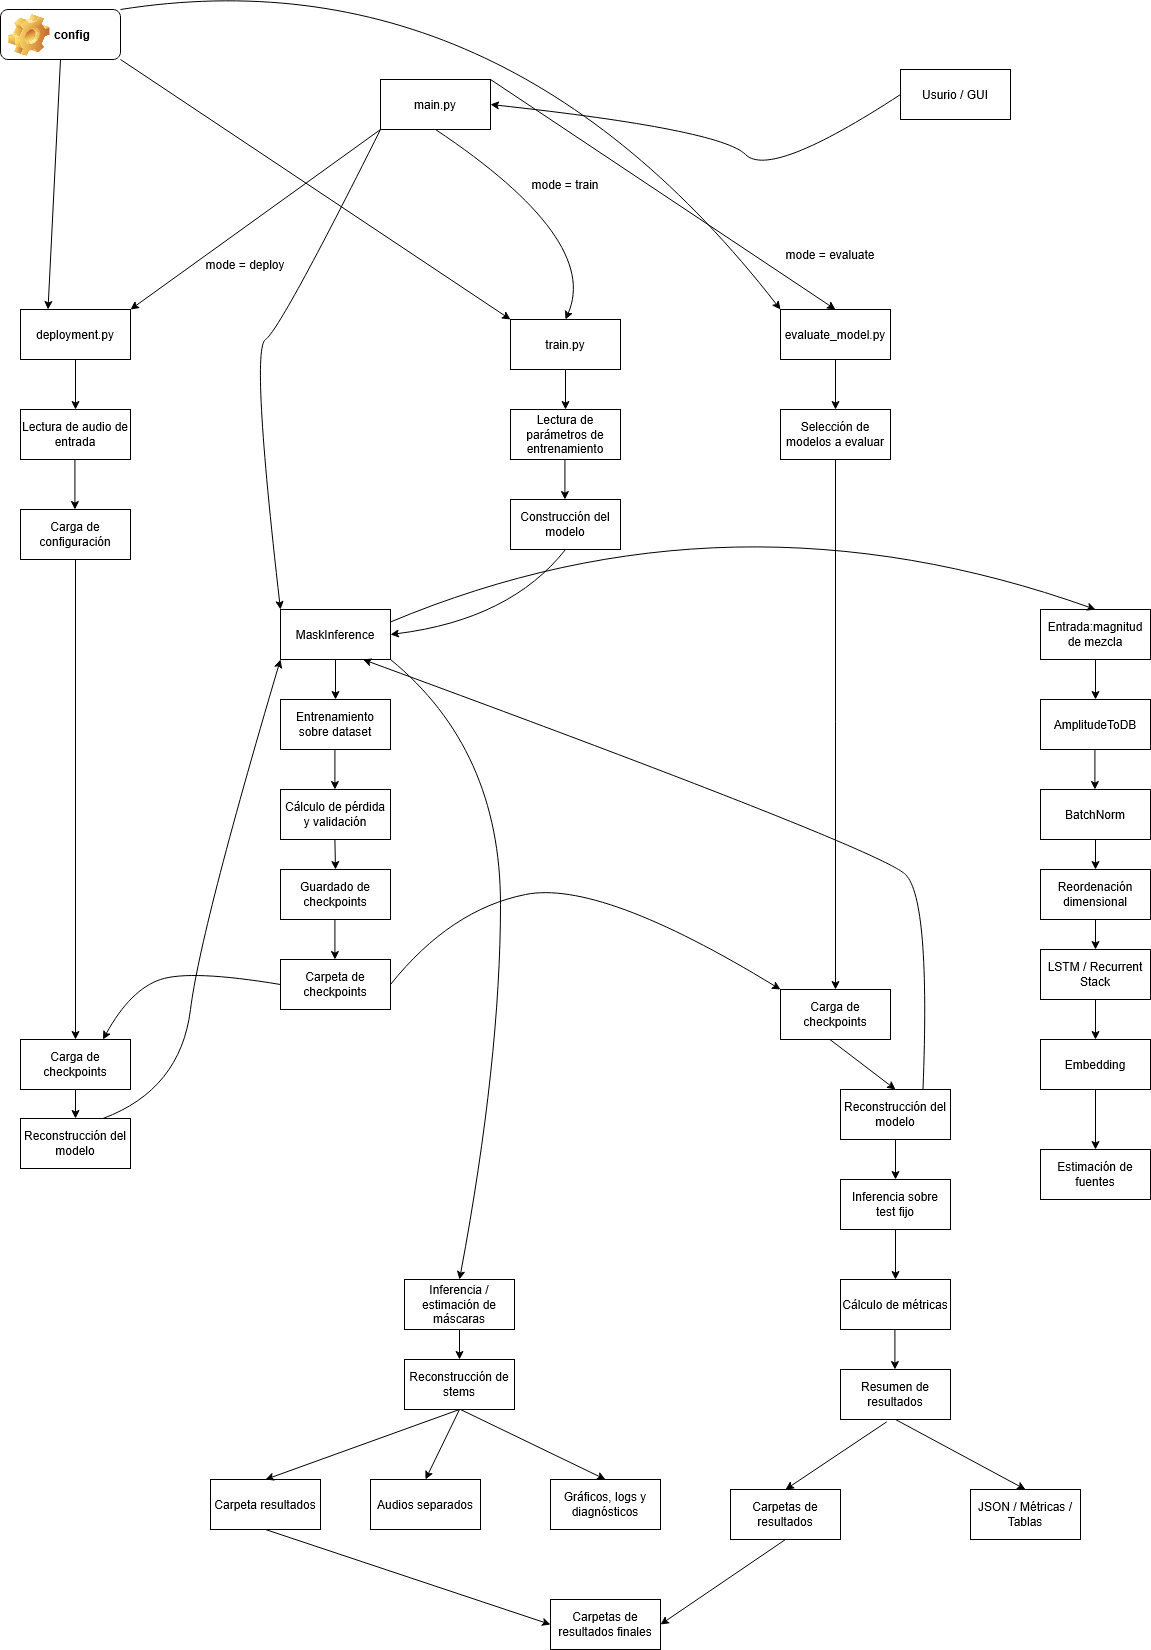
\includegraphics[width=0.7\textwidth]{commons/DiagramaFlujo.png}
    \caption{Diagrama de flujo para el backend}
    \label{fig:DiagramaFlujo}
    \end{center}}
\end{figure}

Y por módulos:

\begin{itemize}
    \item main.py : punto de entrada principal, recibe por comando y ejecuta entrenamiento/despliegue/evaluación
    \item config.py : fuente central de parámetros, entre los que están parámetros de la STFT, hiperparámetros del modelo, función de pérdida, número de fuentes, rutas y dispositivo de ejecución.
    \item train.py : lee la configuración, construye un objeto MaskInference, entrena y calcula el valor de la pérdida y guarda checkpoints en la carpeta correspondiente.
    \item deployment.py : infiere la máscara inferida por el modelo entrenado sobre un audio concreto. Lee un audio de entrada, carga un checkpoint, reconstruye el modelo, ejecuta inferencia, reconstruye las fuentes y guarda los resultados.
    \item evaluate\_models.py : evalúa sistemáticamente los modelos que ya han sido entrenados sobre el conjunto de test fijo. Selecciona modelos, carga sus checkpoints, los reconstruye, ejecuta una separación sobre el conjunto de test, calcula las métricas de evaluación y guarda resúmenes en .json.
    \item MaskInference : contiene la arquitectura del modelo, la llamada a los transformaciones por cada iteración y la función de forward. Toma como entrada la magnitud de mezcla y aplica: AmplitudeToDB,BatchNorm,reordenación dimensional, LSTM/RecurrentStack, Embedding, máscaras estimadas y estimación de fuentes.
    \item Carpetas de checkpoints : guardan los archivos .pth ordenados por función de pérdida y por número de fuentes.
    \item Carpetas de resultados : guardan las salidas del backend. Contienen las fuentes separadas junto con la mezcla original, métricas, gráficos y ficheros resumen.
\end{itemize}

